\documentclass[journal,twoside,web]{ieeecolor}
\usepackage{hyperref}
\usepackage{generic}
\usepackage{cite}
\usepackage{amsmath,amssymb,amsfonts}
\usepackage{algorithmic}
\usepackage{graphicx}
\usepackage{algorithm,algorithmic}
\usepackage{hyperref}
\hypersetup{hidelinks=true}
\usepackage{textcomp}
\def\BibTeX{{\rm B\kern-.05em{\sc i\kern-.025em b}\kern-.08em
    T\kern-.1667em\lower.7ex\hbox{E}\kern-.125emX}}

\title{Supplementary Files}
\author{Arshmeet Kaur}
\date{August 2023}

\begin{document}

\clearpage
\begin{figure*}[!t]
\centering
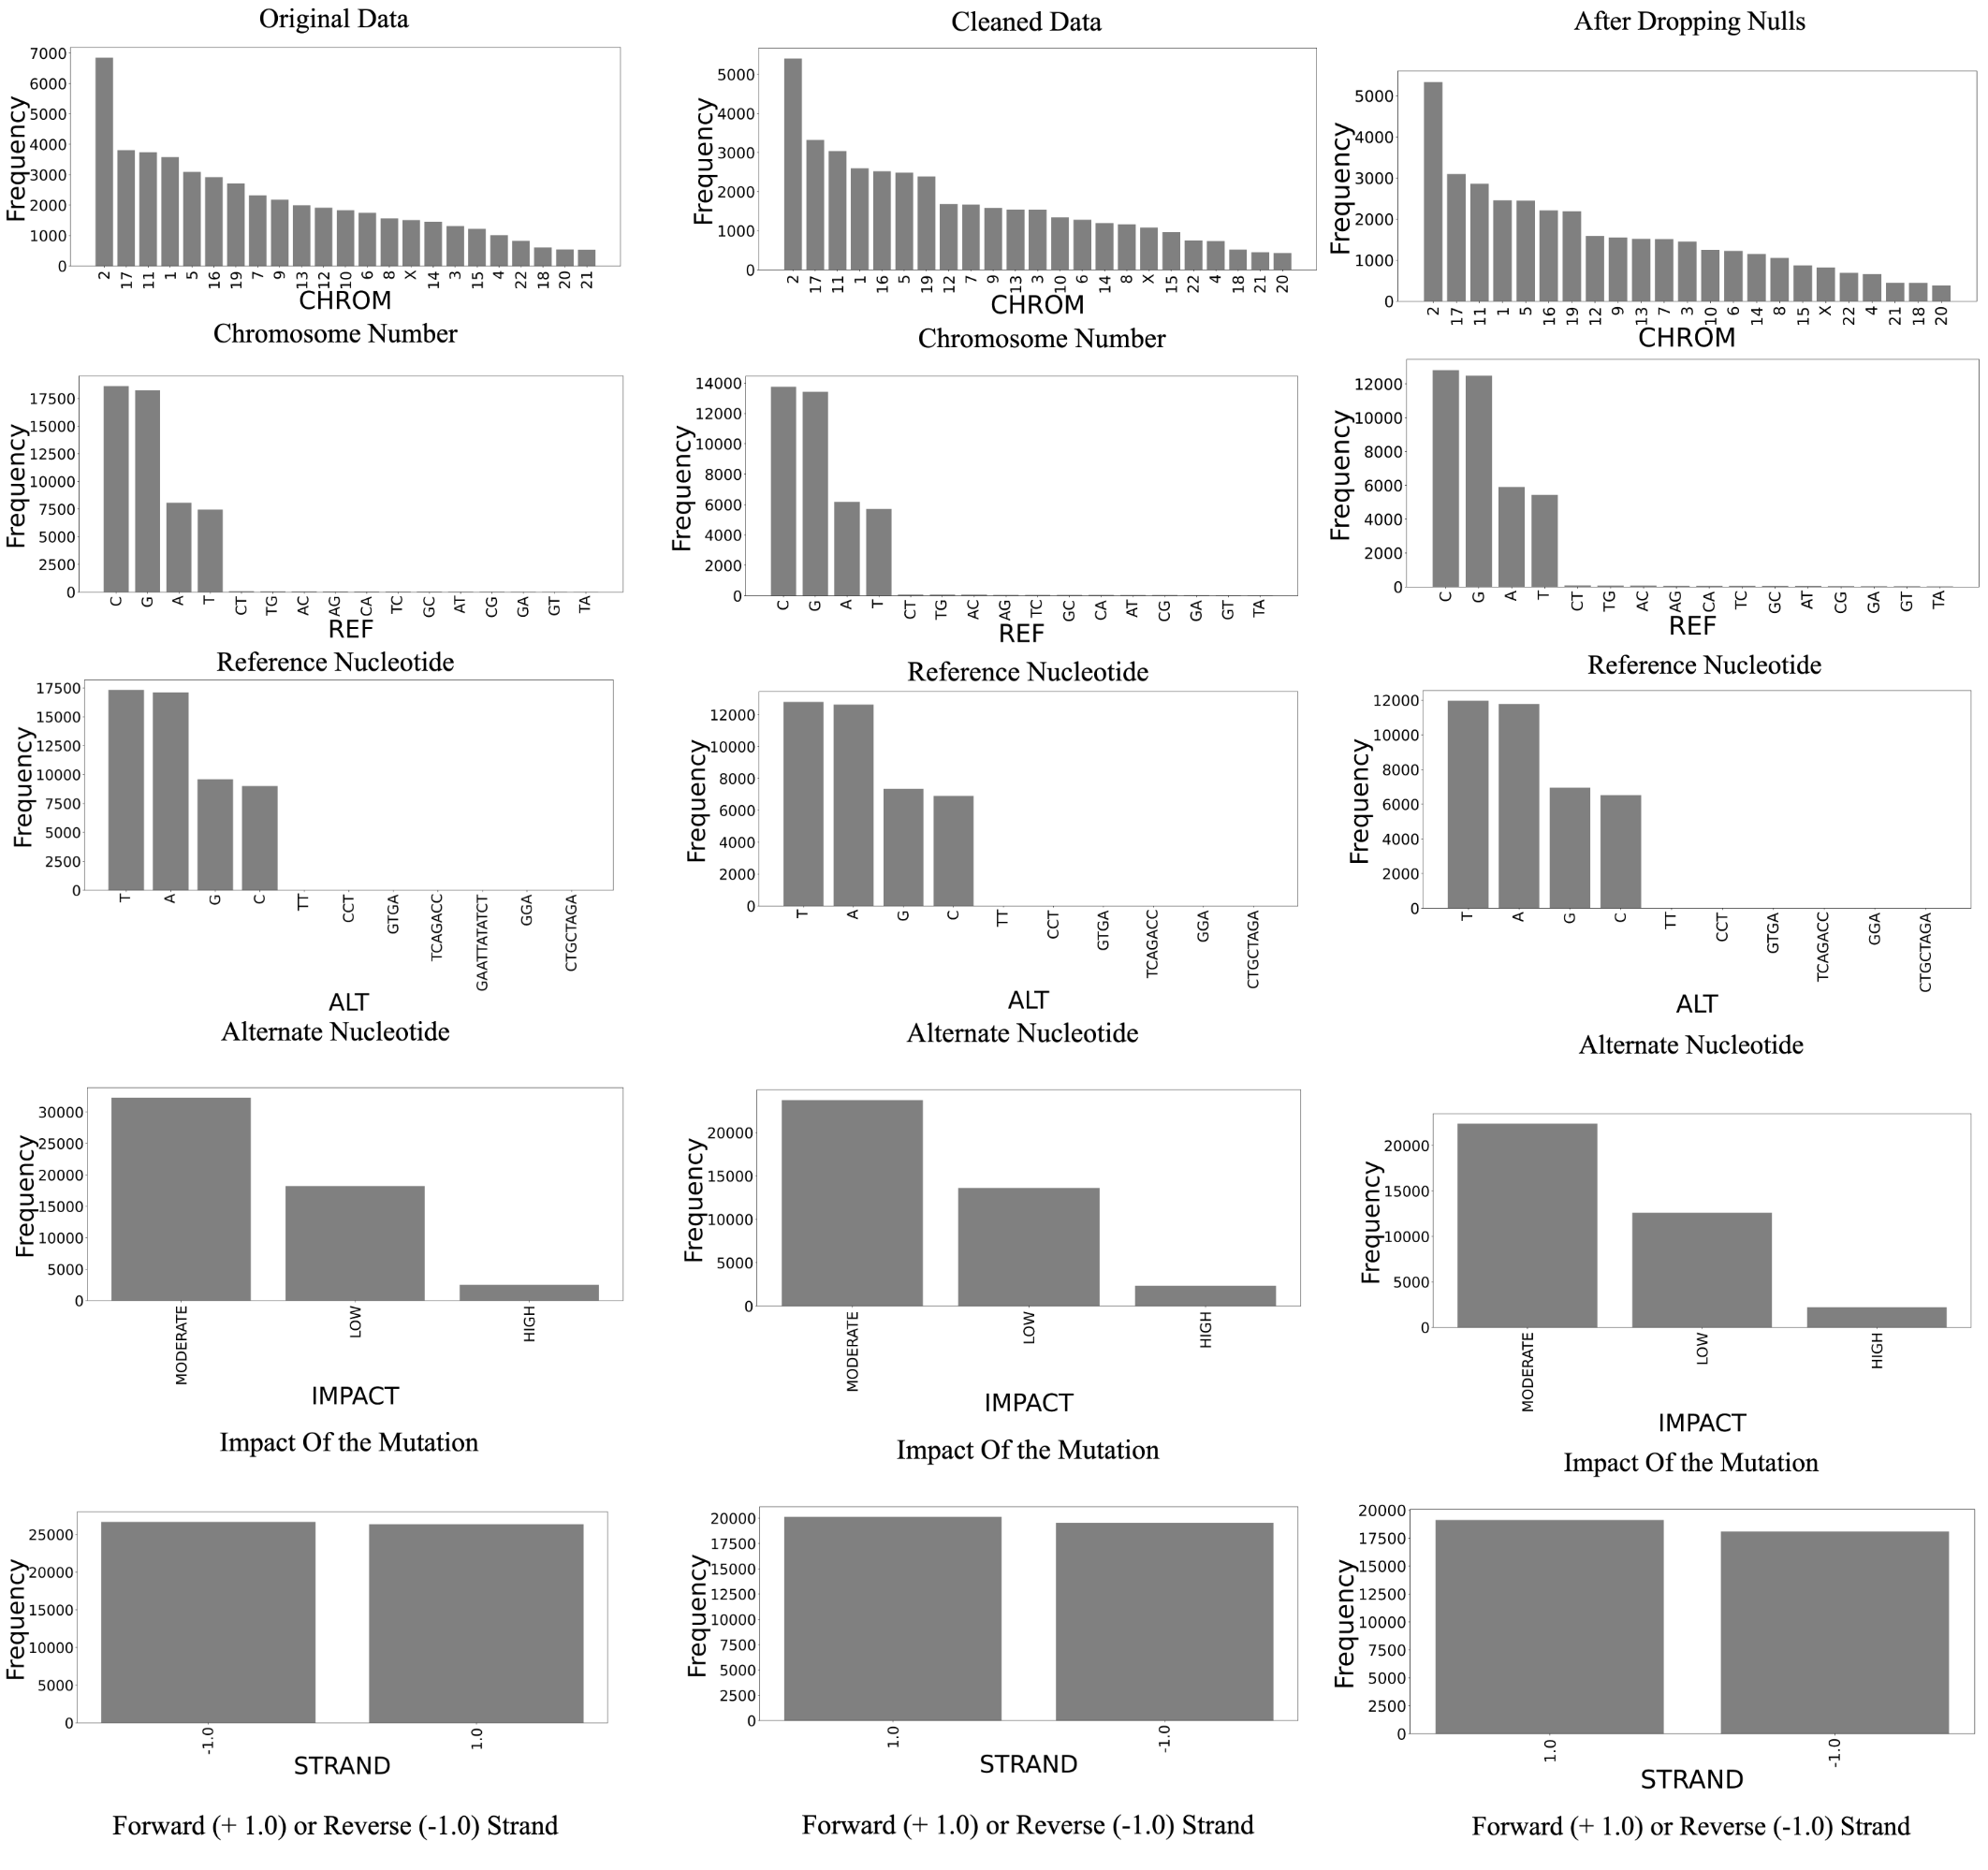
\includegraphics[width=\textwidth]{Supplementary Figure 1 .png}
\caption{Above are categorical variables in the original dataset, and then after data preprocessing (Cleaned Data) and the dropping of all null values for the LoFtool target variable (After Dropping Nulls). Of course, the skew of the data after dropping nulls and encoding values of categorical variables is going to be the same as encoding does nothing to the overall distribution of a variable. If a variable is not included here, it is because it contained too many categories for a meaningful plot. As can be seen, distributions remained similar after every step of data processing.}
\label{fig1}
\end{figure*}

\clearpage
\begin{figure*}[!t]
\centering
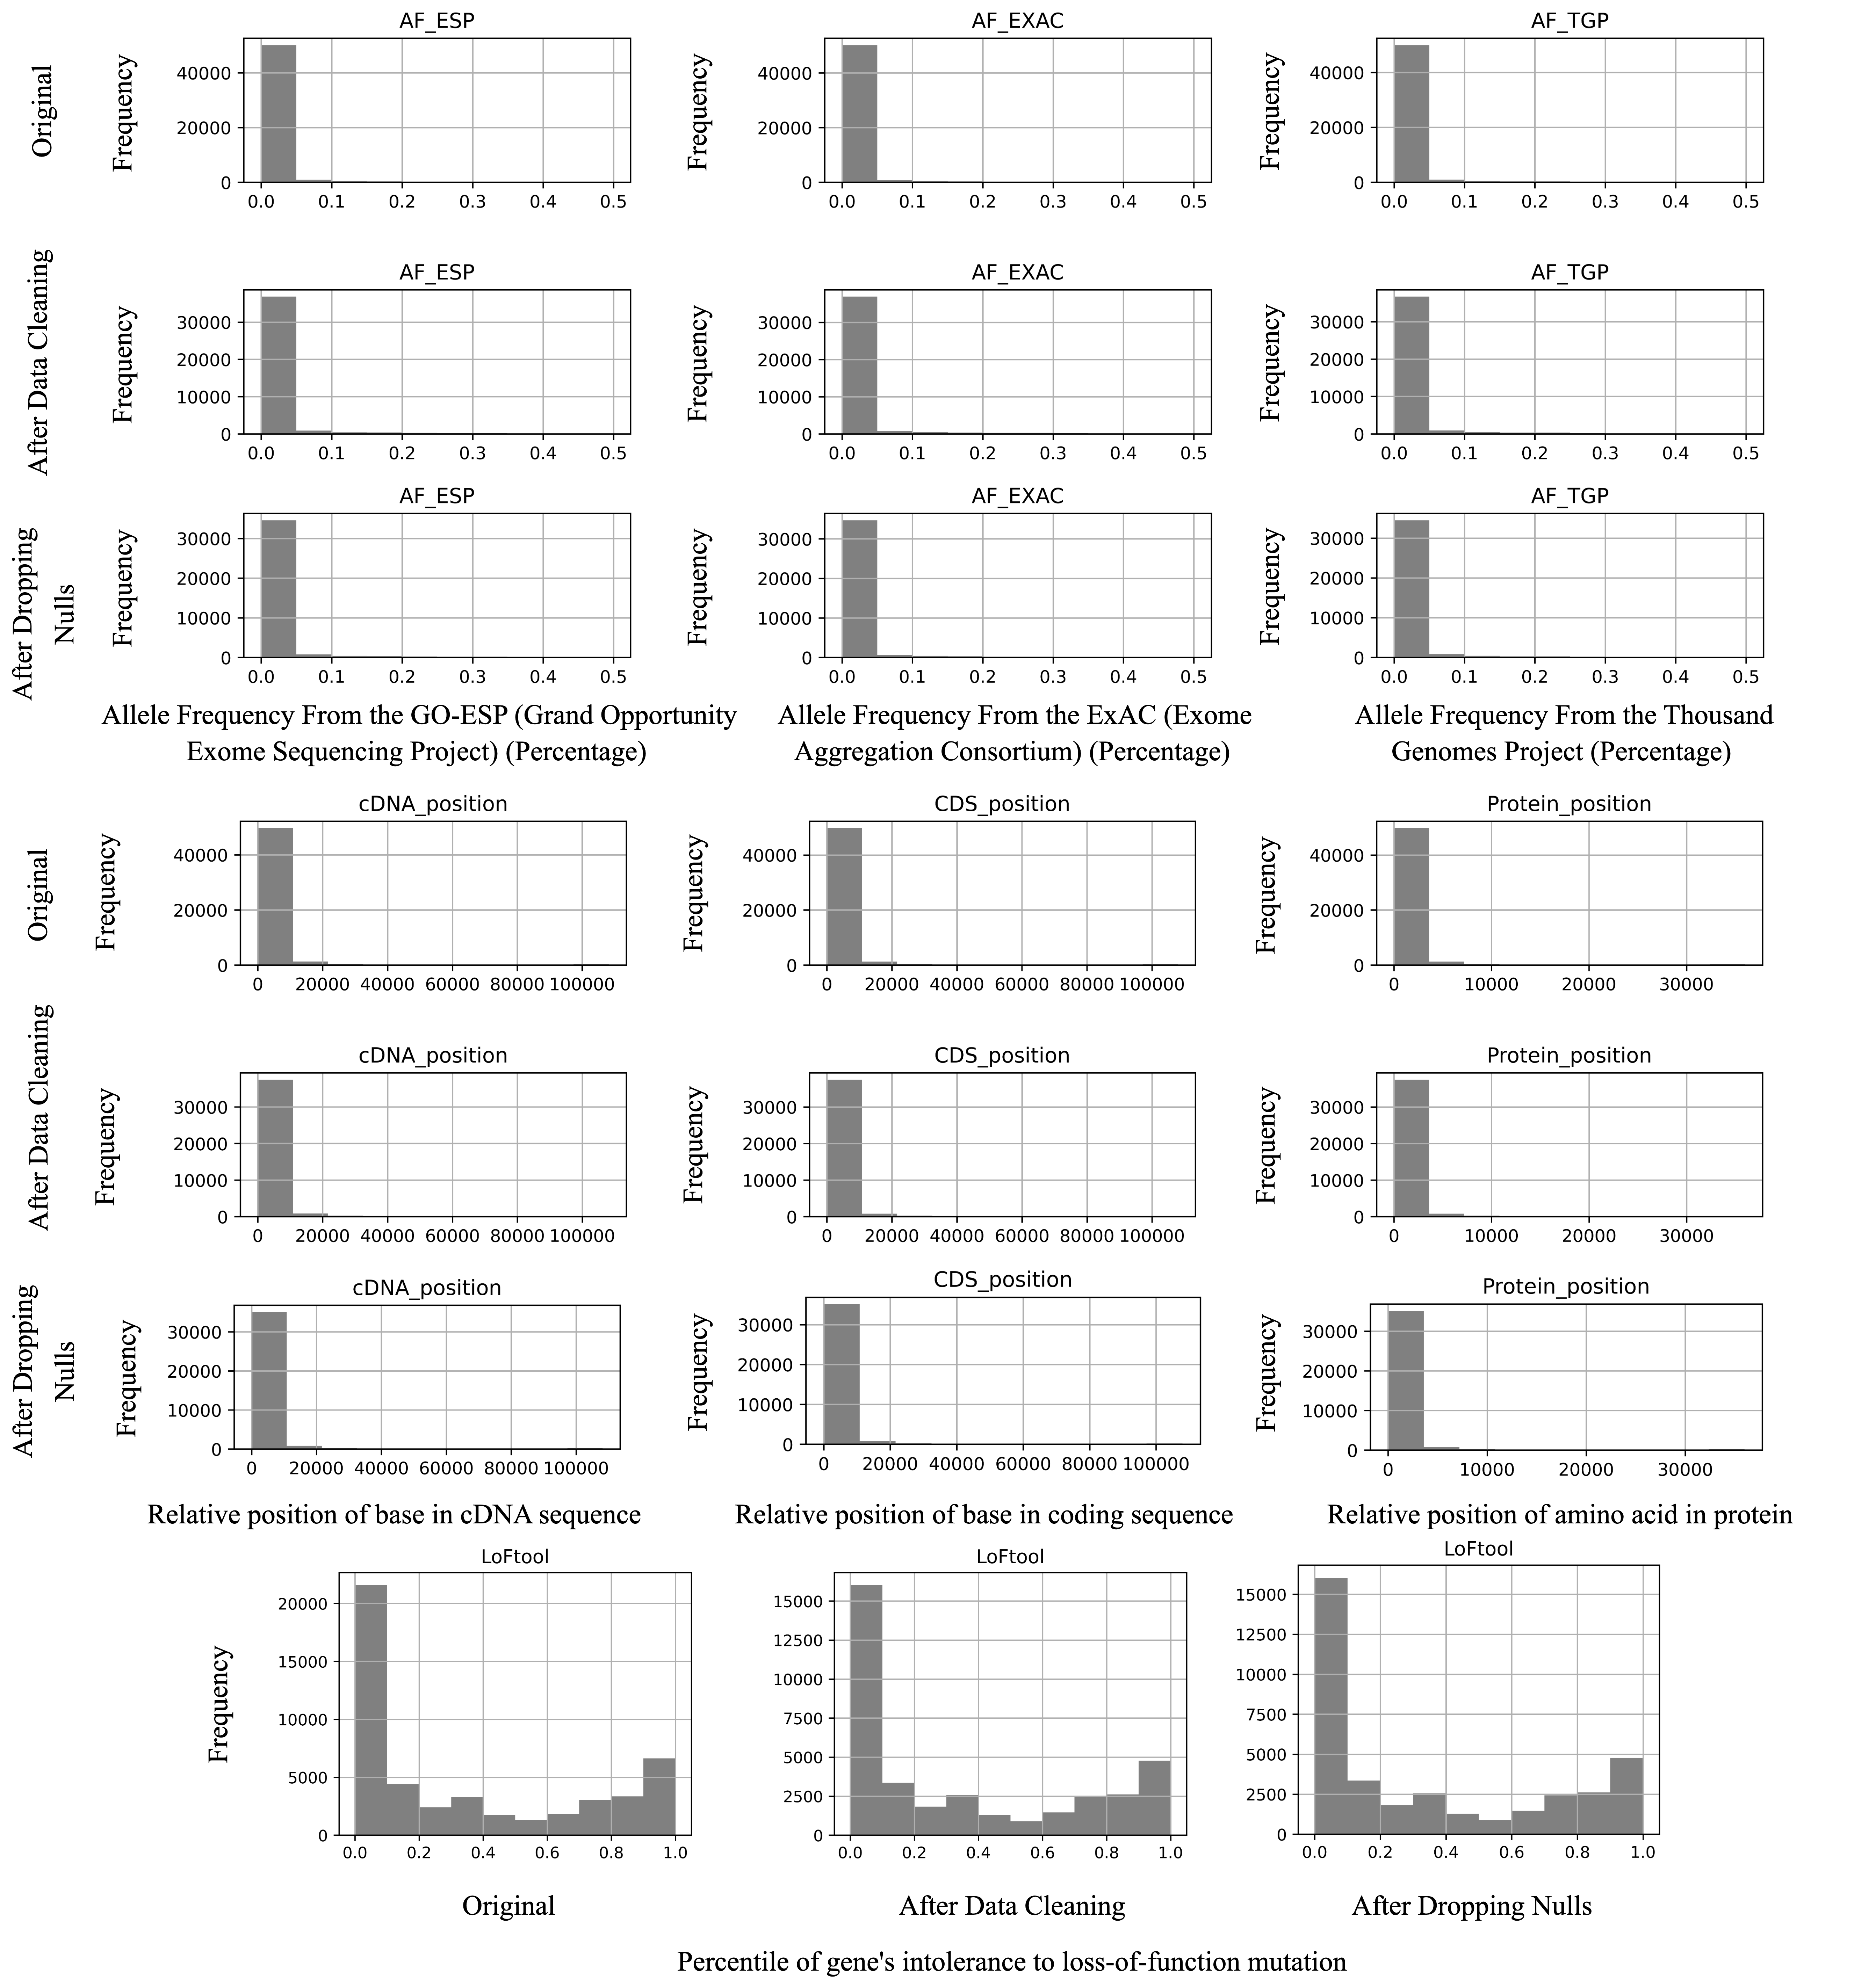
\includegraphics[width=\textwidth]{Supplementary Figure 2 .png}
\caption{Distribution of continuous variables before and after all steps of data preprocessing: original dataset (Original), after data preprocessing/cleaning (After Data Cleaning), and after dropping all nulls for the LoFtool target variable (After Dropping Nulls). All variables retain their heavy right skew after all steps.}
\label{fig2}
\end{figure*}

\end{document}